\documentclass[aspectratio=169]{ctexbeamer} %[t]:顶端对齐
\usetheme{Madrid} %Madrid,蓝色调为主。
\usecolortheme{beaver} %beaver
\usefonttheme{professionalfonts}

\usepackage{universe}
\uBigPaper

\date{\today}
\begin{document}

% 1.2 数轴
\begin{frame}{1.2 数轴}
\begin{definition}
\textbf{\textcolor{orange}{规定了原点、正方向和单位长度的直线叫做数轴(number axis).} } \\
\end{definition}
\vspace{12pt}
\textbf{数轴的四要素:} 
\begin{enumerate}[label={\arabic*.}]
    \item \textbf{原点}
    \item \textbf{正方向}
    \item \textbf{单位长度}
    \item \textbf{直线(强调三要素的只包括前三条)}
\end{enumerate}
\vspace{24pt}
\textbf{\textcolor{blue} {数轴示例:}}
\vspace{24pt}
\begin{figure}
\fontsize{20}{24}\selectfont
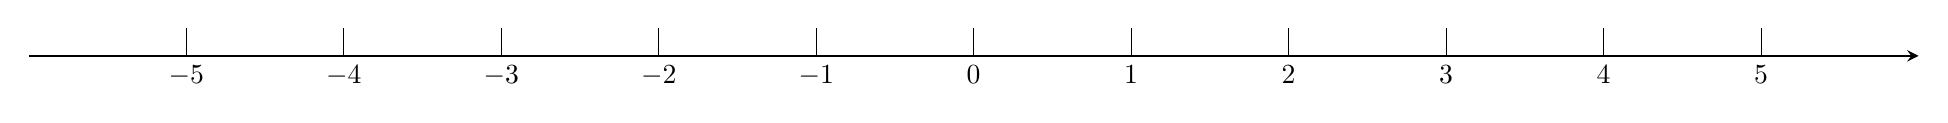
\begin{tikzpicture}[scale=2]
\draw [black, thick, ->, >=stealth] (-6,0) -- (6,0); 
\foreach \x in {-5, ..., 5}
	\draw (\x cm,5pt) -- (\x cm,0pt) node[anchor=north] {$\x$};
\end{tikzpicture}
\end{figure}
\end{frame}

\begin{frame}{最简数轴}
\begin{definition}
\textbf{\textcolor{orange}{规定了原点、正方向和单位长度的直线叫做数轴(number axis).} } \\
\end{definition}
\vspace{12pt}
\vspace{1cm}
\textbf{以下图形是不是一个数轴?}
\vspace{1cm}
\begin{figure}
\fontsize{20}{24}\selectfont
\begin{tikzpicture}[scale=2]
\draw [black, thick, -stealth] (-4,0) -- (4,0); 
\foreach \x in {0, 1}
 	\draw (\x cm,5pt) -- (\x cm,0pt) node[anchor=north] {$\x$};
\end{tikzpicture} 
\end{figure}
\end{frame}

\begin{frame}{类比思维}
\textbf{\textcolor{orange}{规定了原点、正方向和单位长度的直线叫做数轴(number axis).} } 
\begin{figure}
\fontsize{20}{24}\selectfont
\begin{tikzpicture}

\coordinate (A) at (-5, 0);
\coordinate (B) at (-3, 0);
\coordinate (C) at (-2, 0);
\coordinate (D) at (2,0);
\coordinate (D1) at (5, 0);

\coordinate (E1) at (-5, -2);
\coordinate (F1) at (5, -2);
\coordinate (E) at (-2, -2);
\coordinate (F) at (2, -2);
\draw [Circle-Circle] (A) node [below] {A} -- node [above =0.1cm] {线段AB} (B) [below] node {B}; %画线段
%画射线
\draw [Circle-] (C) node [below] {C} -- node  [above=0.1cm] {射线CD}  (D1);
\fill (D) circle(2pt) node [below] {D}; 
 %画直线
\draw (E1)  --node  [above=0.1cm] {直线EF} (F1);
\fill (E) circle(2pt) node [below] {E}  (F) circle(2pt) node [below] {F};

\end{tikzpicture}
\end{figure}
【北京师范大学四年级上册(2013)P16】\\
\textbf{线段:线段有两个端点,线段有一定的长度。} \\
\textbf{射线:射线有一个端点,射线可以向一个方向无限延伸。} \\
\textbf{直线:直线没有端点,直线可以向两个方向无限延伸。} \\
\begin{figure}
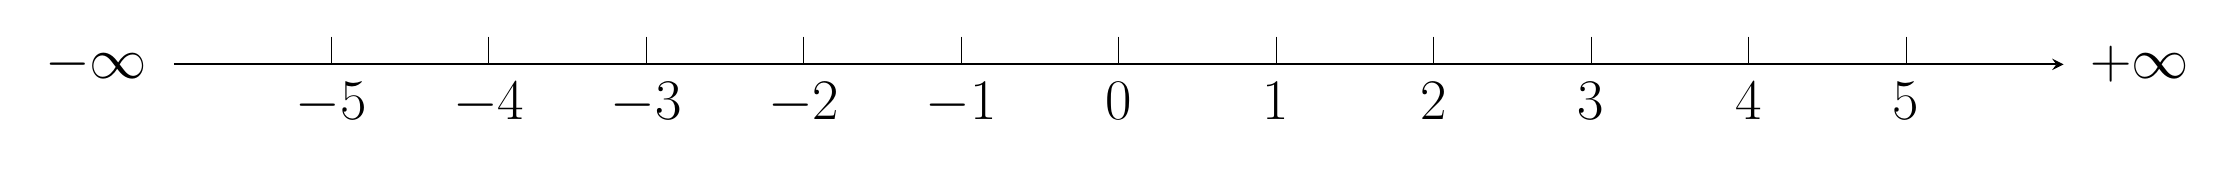
\begin{tikzpicture}[scale=2]
\fontsize{20}{24}\selectfont
\draw [black, thick, -stealth] (-6,0) node [left=0.1cm] {$-\infty$} -- (6,0) node [right=0.1cm] {+$\infty$}; 
\foreach \x in {-5,...,5}
 	\draw (\x cm,5pt) -- (\x cm,0pt) node[anchor=north] {$\x$};
\end{tikzpicture} 
\end{figure}
\textbf{实数集$\mathbb{R}$可以用区间表示为$(-\infty, +\infty)$,$\infty$读作“无穷大”,“$-\infty$”读作“负无穷大”,“$+\infty$”读作“正无穷大”.【必修A版一册P64】}
\end{frame}

\end{document}